% !TeX spellcheck = de_AT_frami
\documentclass[10pt,a4paper]{article}
\usepackage[utf8x]{inputenc}
\usepackage{ucs}
\usepackage{amsmath}
\usepackage{setspace}
\usepackage{amsfonts}
\usepackage{amssymb}
\usepackage{graphicx}
\usepackage{txfonts}
\usepackage[dvipsnames]{xcolor}
\usepackage{geometry}
\usepackage{graphicx}
\usepackage{epstopdf}
\epstopdfsetup{update}
\geometry{margin= 2cm}
\usepackage[makeroom]{cancel}
\usepackage{multirow}
\setlength\parindent{0pt}

\usepackage{scalerel,stackengine}
\stackMath
\newcommand\reallywidehat[1]{%
	\savestack{\tmpbox}{\stretchto{%
			\scaleto{%
				\scalerel*[\widthof{\ensuremath{#1}}]{\kern-.6pt\bigwedge\kern-.6pt}%
				{\rule[-\textheight/2]{1ex}{\textheight}}%WIDTH-LIMITED BIG WEDGE
			}{\textheight}% 
		}{0.5ex}}%
	\stackon[1pt]{#1}{\tmpbox}%
}
\parskip 1ex


\begin{document}
	\pagenumbering{gobble}
	\section*{6. Numerik Übungen 2017/18}
	\paragraph{T9}\mbox{}\\
	\textbf{%
		a) Prüfen Sie nach, ob die Formel (3.38) für die Lagrange-Polynome $\pmb{l_1}$ wirklich die Bedingung $\pmb{l_i(x_j)=\delta_{ij}}$ erfüllt.
	}\\
	S. 47
	\begin{align}\tag{3.37}
	l_i(x_j)=\delta_{ij} =
	\begin{cases}
	1, & \text{falls } i=j,\\
	0, & \text{falls } i\neq j.
	\end{cases} \nonumber
	\end{align}
	\begin{align}\tag{3.38}
	l_i(x)=\frac{(x-x_0)(x-x_1)\cdots\reallywidehat{(x-x_i)}\cdots(x-x_n)}{(x_i-x_0)(x_i-x_1)\cdots\reallywidehat{(x_i-x_i)}\cdots(x_i-x_n)}
	\end{align}
	\begin{align*}
	i=j, &\quad l_i(x_i)=\frac{\cancel{(x_i-x_0)}\cancel{(x_i-x_1)}\cdots\bcancel{\cancel{\reallywidehat{(x_i-x_i)}}}\cdots\cancel{(x_i-x_n)}}{\cancel{(x_i-x_0)}\cancel{(x_i-x_1)}\cdots\bcancel{\cancel{\reallywidehat{(x_i-x_i)}}}\cdots\cancel{(x_i-x_n)}} = 1\\
	i\neq j, &\quad l_i(x_j)=0 \Rightarrow (x_j-x_0)(x_j-x_1)\cdots\bcancel{\cancel{\reallywidehat{(x_j-x_i)}}}\cdots(x_j-x_n) \overset{!}{=} 0 \\
	& \quad \text{Wahr, wenn } x_j \in x
	\end{align*}
	\textbf{%
		b) Interpolieren Sie $\pmb{f(x)=6-4x+\frac{1}{2}x^3}$ an den Stützstellen $\pmb{x_k=k-3, k=0,\dots ,5}$, durch eine stückweise lineare Funktion $\pmb{s}$. Geben Sie dazu die gesuchte stückweise lineare Funktion $\pmb{s}$ als Linearkombination 
		\begin{align*}
		\pmb{s(x) = \sum_{k=0}^{5}y_k\phi_k(x)}
		\end{align*}
		von Hutfunktionen $\pmb{\phi_k(x)}$ an. \\
		Sie brauchen die Hutfunktionen $\pmb{\phi_k(x)}$ nicht explizit anzugeben, eine Skizze mit der Funktion $\pmb{f}$, der Interpolierenden $\pmb{s}$, allen auftretenden Hutfunktionen $\pmb{\phi_k(x)}$ und Vielfachen $\pmb{y_k\phi_k(x)}$ (mit Nummerierung) ist ausreichend. 
	}	\\
	S. 59
	\begin{alignat*}{8}
	x =& \begin{bmatrix}-3 & -2 & -1 &0& 1& 2 \end{bmatrix}, \qquad s(x)=\sum_{i=0}^{n}y_i\phi_i(x)
	\end{alignat*}
	\begin{align*}
	\phi_i(x) &= \begin{cases}
	\frac{x-x_{i-1}}{x_i-x_{i-1}}, \; x \in [x_{i-1}, x_i] & \text{falls } i=1,\dots, n\\
	\frac{x_{i+1}-x}{x_{i+1}-x_i}, \; x \in [x_i, x_{i+1}] & \text{falls } i=0,\dots, n-1\\
	\quad 0, & \text{sonst}
	\end{cases} \\
	\phi_0(x) &= \begin{cases}
	\frac{x_{1}-x}{x_{1}-x_0}, & x \in [x_0, x_{1}] \\
	\quad\! 0, & \text{sonst}
	\end{cases} =
	\begin{cases}
	\frac{-2-x}{-2+3}, & x \in [-3, -2] \\
	\quad\! 0, & \text{sonst}
	\end{cases}
	\\
	\phi_2(x) &= \begin{cases}
	\frac{x-x_{1}}{x_2-x_{1}}, & x \in [x_{1}, x_2] \\
	\frac{x_{3}-x}{x_{3}-x_2}, & x \in [x_2, x_{3}] \\
	\quad 0, & \text{sonst}
	\end{cases}
	= \begin{cases}
	\frac{x+2}{-1+2}, & x \in [-2, -1]\\
	\:\frac{0-x}{0+1}, & x \in [-1, \;\;\,0] \\
	\quad 0, & \text{sonst}
	\end{cases}
	\end{align*}
	\begin{figure}[htbp]
		\centering
		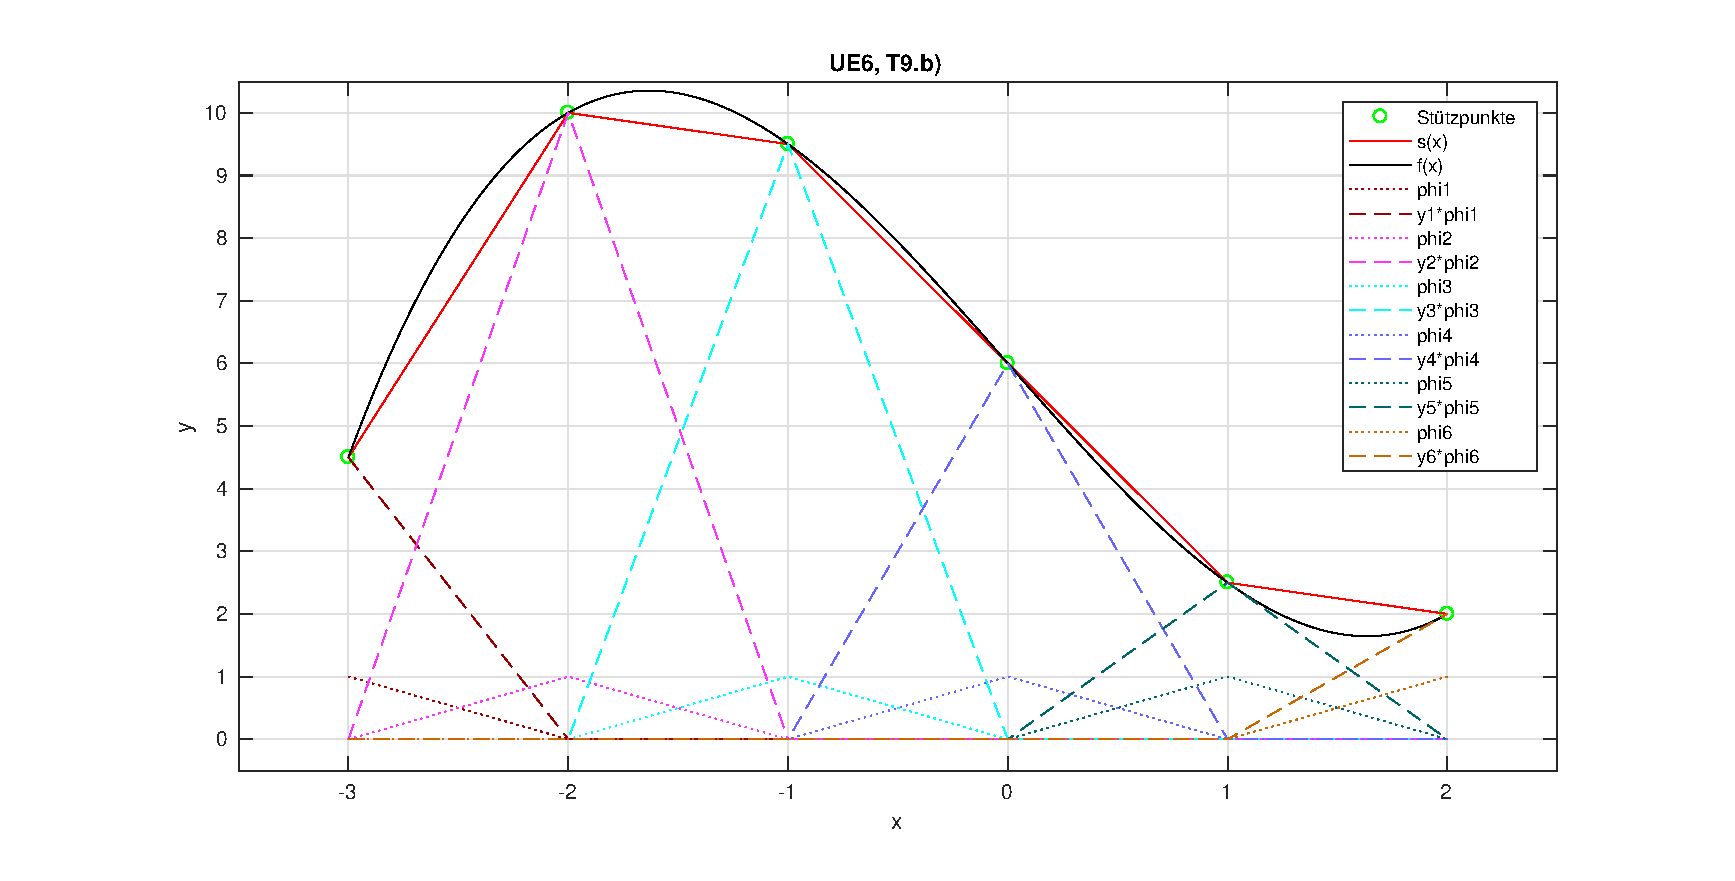
\includegraphics[width=1.0\textwidth]{T9b}
		\caption{T9.b \, Stützpunkte, Funktion $f$, Stückweise lineare Interpolation $s$, Hutfunktionen ohne und mit Skalierung.}
	\end{figure}
	
	
	\clearpage
	
	
	\paragraph{T10}\mbox{}\\
	\textbf{%
		Gegeben sind die Punkte $\pmb{(x_0,y_0)=(-1,2)}$, $\pmb{(x_1,y_1)=(0,3)}$ und $\pmb{(x_2,y_2)=(1,3)}$ sowie die Ableitungen $\pmb{y'_0=3}$, $\pmb{y'_1=2}$, $\pmb{y'_2=-3}$ und $\pmb{y''_1=4}$.\\
		Bestimmen Sie ein Polynom $\pmb{p}$, sodass $\pmb{p(x_i)=y_i}$, $\pmb{p'(x_i)=y'_i}$, $\pmb{i=0,1,2}$, und $\pmb{p''(x_1)=y''_1}$.\\
		Zeichnen Sie das Polynom $\pmb{p}$ und die Punkte in {\scshape Matlab}.
	}\\
	S. 54 \\
	Allgemeines Differenzenschema für Hermite-Interpolation mit gegebenen Ableitungen vom Grad 2
	\begin{align*}
	\begin{array}{ll|c}
		x_i                   & y_i                       &                        \delta y_i                        \\ \hline
		x_0                   & y_0                       &  \\
		                      &                           &          \frac{y_0+hy'_0-y_0}{x_0+h-x_0} = y'_0          \\
		x_0+h \rightarrow x_0 & y_0+hy'_0 \rightarrow y_0 &  \\
		                      &                           & \frac{y_1-(y_0+hy'_0)}{x_1-(x_0+h)}\rightarrow\delta y_0 \\
		x_1                   & y_1                       &  \\
		                      &                           &          \frac{y_1+hy'_1-y_1}{x_1+h-x_1} = y'_1          \\
		x_1+h \rightarrow x_1 & y_1+hy'_1 \rightarrow y_1 &  \\
		\vdots                & \vdots                    &                          \vdots
	\end{array} \rightarrow
		\begin{array}{ll|c}
			x_i    & y_i    & \delta y_i \\ \hline
			x_0    & y_0    &  \\
			       &        &    y'_0    \\
			x_0    & y_0    &  \\
			       &        & \delta y_0 \\
			x_1    & y_1    &  \\
			       &        &    y'_1    \\
			x_1    & y_1    &  \\
			\vdots & \vdots &   \vdots
		\end{array}
	\end{align*}
	\begin{align*}
		x = \begin{bmatrix}-1 & 0 & 1\end{bmatrix},\quad y = \begin{bmatrix}2 & 3 & 3\end{bmatrix} ,\quad y'_0 = 3,\quad y'_1 = 2,\quad y_2'=-3,\quad y''_1=4
	\end{align*}
	 Ausgehend vom Differenzenschema für das Newtonsche Interpolationspolynom \\
	 Schritt 1: Vermehrung der Stützstellen, einmal je gegebenen Ableitungsgrad je Stützstelle, hier +1 für $x_0, x_2$ und +2 für $x_1$.
	 \begin{align*}
		 \begin{array}{cc|cccc}
		 	x_i & y_i &  &  &  \\ \hline
		 	x_0 & y_0 &  &  \\
		 	    &     &  &  \\
		 	x_0 & y_0 &  &  \\
		 	    &     &  &  \\
		 	x_1 & y_1 &  &  \\
		 	    &     &  &  \\
		 	x_1 & y_1 &  &  \\
		 	    &     &  &  \\
		 	x_1 & y_1 &  &  \\
		 	    &     &  &  \\
		 	x_2 & y_2 &  &  \\
		 	    &     &  &  \\
		 	x_2 & y_2 &
		 \end{array}
	        \rightarrow
			\begin{array}{cc|cccc}
				x_i & y_i &  &  &  \\ \hline
				-1  &  2  &  &  \\
				    &     &  &  \\
				-1  &  2  &  &  \\
				    &     &  &  \\
				 0  &  3  &  &  \\
				    &     &  &  \\
				 0  &  3  &  &  \\
				    &     &  &  \\
				 0  &  3  &  &  \\
				    &     &  &  \\
				 1  &  3  &  &  \\
				    &     &  &  \\
				 1  &  3  &  &
			\end{array}
		\end{align*}
	\newpage
	Schritt 2: Berechnung des Differenzenschema \\
	Wie gewohnt mit der Merkregel des Newtonschen Interpolationspolynom (S. 38) \\
	Bleibt nach dem Grenzübergang $h \rightarrow 0$ nur $\frac{0}{0}$ muss der Wert mit einer bekannten Ableitung in der Form $\frac{f^{(g)}(x)}{g!}$ ersetzt werden.
	
	\begin{align*}
		\begin{array}{rr|lccc}
			x_i & y_i & \delta y_i &  &  \\ \hline
			x_0 & y_0 &  &  \\
			    &     & \frac{y_0-y_0}{x_0-x_0}=\frac{0}{0}\rightarrow y'_0 &  \\
			x_0 & y_0 &  &  \\
			    &     & \frac{y_1-y_0}{x_1-x_0}=\delta y_0 &  \\
			x_1 & y_1 &  &  \\
			    &     & \frac{y_1-y_1}{x_1-x_1}=\frac{0}{0}\rightarrow y'_1 &  \\
			x_1 & y_1 &  &  \\
			    &     & \frac{y_1-y_1}{x_1-x_1}=\frac{0}{0}\rightarrow y'_1 &  \\
			x_1 & y_1 &  &  \\
			    &     & \frac{y_2-y_1}{x_2-x_1}=\delta y_1 &  \\
			x_2 & y_2 &  &  \\
			    &     & \frac{y_2-y_2}{x_2-x_2}=\frac{0}{0}\rightarrow y'_2 &  \\
			x_2 & y_2 &
		\end{array}
			\rightarrow
				\begin{array}{cc|rccc}
					x_i & y_i &  &  &  \\ \hline
					-1  &  2  &  &  \\
					    &     & 3 &  \\
					-1  &  2  &  &  \\
					    &     & \frac{3-2}{0+1}=1 &  \\
					 0  &  3  &  &  \\
					    &     & 2 &  \\
					 0  &  3  &  &  \\
					    &     & 2 &  \\
					 0  &  3  &  &  \\
					    &     & \frac{3-3}{1-0}=0 &  \\
					 1  &  3  &  &  \\
					    &     & -3 &  \\
					 1  &  3  &  &
				\end{array}
	\end{align*}
	Hier also $\frac{f^{(2)}(x_1)}{2!}$
	\begin{align*}
		\begin{array}{rr|llcc}
			x_i & y_i & \delta y_i & \delta^2 y_i &  \\ \hline
			x_0 & y_0 &            &  \\
			    &     & y'_0       &  \\
			x_0 & y_0 &            & \frac{\delta y_0-y'_0}{x_1-x_0} \\
			    &     & \delta y_0 &  \\
			x_1 & y_1 &            & \frac{y'_1 - \delta y_0}{x_1-x_0} \\
			    &     & y'_1       &  \\
			x_1 & y_1 &            & \frac{y'_1-y'_1}{x_1-x_1}=\frac{0}{0}\rightarrow \frac{y''_1}{2!} \\
			    &     & y'_1       &  \\
			x_1 & y_1 &            & \frac{\delta y_1-y'_1}{x_2-x_1} \\
			    &     & \delta y_1 &  \\
			x_2 & y_2 &            & \frac{y'_2 - \delta y_1}{x_2-x_1} \\
			    &     & y'_2       &  \\
			x_2 & y_2 &
		\end{array}
			\rightarrow
				\begin{array}{cc|rrcc}
					x_i & y_i &  \delta y_i  & \delta^2 y_i &  \\ \hline
					-1  &  2  &    &  \\
					    &     &  3 &  \\
					-1  &  2  &    & \frac{1-3}{0+1}=-2 \\
					    &     &  1 &  \\
					 0  &  3  &    & \frac{2-1}{0+1}=1 \\
					    &     &  2 &  \\
					 0  &  3  &    &  \frac{4}{2}=2 \\
					    &     &  2 &  \\
					 0  &  3  &    & \frac{0-2}{1-0}=-2 \\
					    &     &  0 &  \\
					 1  &  3  &    & \frac{-3-0}{1-0}=-3 \\
					    &     & -3 &  \\
					 1  &  3  &    &
				\end{array}
	\end{align*}
	Rest wie bekannt aus UE5 T7
	\begin{align*}
		\begin{array}{cc|rrrrrr}
			x_i & y_i & \delta y_i & \delta^2 y_i & \delta^3y_i & \delta^4y_i &  \delta^5y_i & \delta^6y_i \\ \hline
			-1  &  2  &            &  \\
			    &     &          3 &  \\
			-1  &  2  &            &           -2 &  \\
			    &     &          1 &              &           3 &  \\
			 0  &  3  &            &            1 &             &          -2 &  \\
			    &     &          2 &              &           1 &             & -\frac{1}{4} &  \\
			 0  &  3  &            &            2 &             &        -2.5 &              & \frac{3}{2} \\
			    &     &          2 &              &          -4 &             &         2.75 &  \\
			 0  &  3  &            &           -2 &             &           3 &  \\
			    &     &          0 &              &          -1 &  \\
			 1  &  3  &            &           -3 &  \\
			    &     &         -3 &  \\
			 1  &  3  &            &
		\end{array}
	\end{align*}
	Hinzufügen der benötigten Stützstellen
	\begin{align*} \hspace{-1cm} {\small
	\begin{array}{cc|rrrrrr}
		x_i &    y_i     &       \delta y_i &          \delta^2 y_i &                \delta^3y_i &                       \delta^4y_i &                            \delta^5y_i &                                 \delta^6y_i \\ \hline
		-1  & 2,\, [x_0] &                  &  \\
		    &            &  3,\, [x_0, x_0] &  \\
		-1  & 2,\, [x_0] &                  & -2,\, [x_0, x_0, x_1] &  \\
		    &            &  1,\, [x_0, x_1] &                       &  3,\, [x_0, x_0, x_1, x_1] &  \\
		 0  & 3,\, [x_1] &                  &  1,\, [x_0, x_1, x_1] &                            &   -2,\, [x_0, x_0, x_1, x_1, x_1] &  \\
		    &            &  2,\, [x_1, x_1] &                       &  1,\, [x_0, x_1, x_1, x_1] &                                   & -\frac{1}{4},\, [x_0, x_0, x_1, x_1, x_1, x_2] &  \\
		 0  & 3,\, [x_1] &                  &  2,\, [x_1, x_1, x_1] &                            & -2.5,\, [x_0, x_1, x_1, x_1, x_2] & & \frac{3}{2},\, [x_0, x_0, x_1, x_1, x_1, x_2, x_2] \\
		    &            &  2,\, [x_1, x_1] &                       & -4,\, [x_1, x_1, x_1, x_2] &                                   & 2.75,\, [x_0, x_1, x_1, x_1, x_2, x_2] &  \\
		 0  & 3,\, [x_1] &                  & -2,\, [x_1, x_1, x_2] &                            &    3,\, [x_1, x_1, x_1, x_2, x_2] &  \\
		    &            &  0,\, [x_1, x_2] &                       & -1,\, [x_1, x_1, x_2, x_2] &  \\
		 1  & 3,\, [x_2] &                  & -3,\, [x_1, x_2, x_2] &  \\
		    &            & -3,\, [x_2, x_2] &  \\
		 1  & 3,\, [x_2] &                  &
	\end{array} }
	\end{align*}
	Daraus ergibt sich analog zu S. 55 das Polynom
	\begin{align*}
		p(x) &= (((((\frac{3}{2}(x-x_2)-\frac{1}{4})(x-x_1)-2)(x-x_1)+3)(x-x_1)-2)(x-x_0)+3)(x-x_0)+2 \\
			 &= (((((\frac{3}{2}(x-1)-\frac{1}{4})(x-0)-2)(x-0)+3)(x-0)-2)(x+1)+3)(x+1)+2
	\end{align*}
	\begin{figure}[htbp]
		\centering
		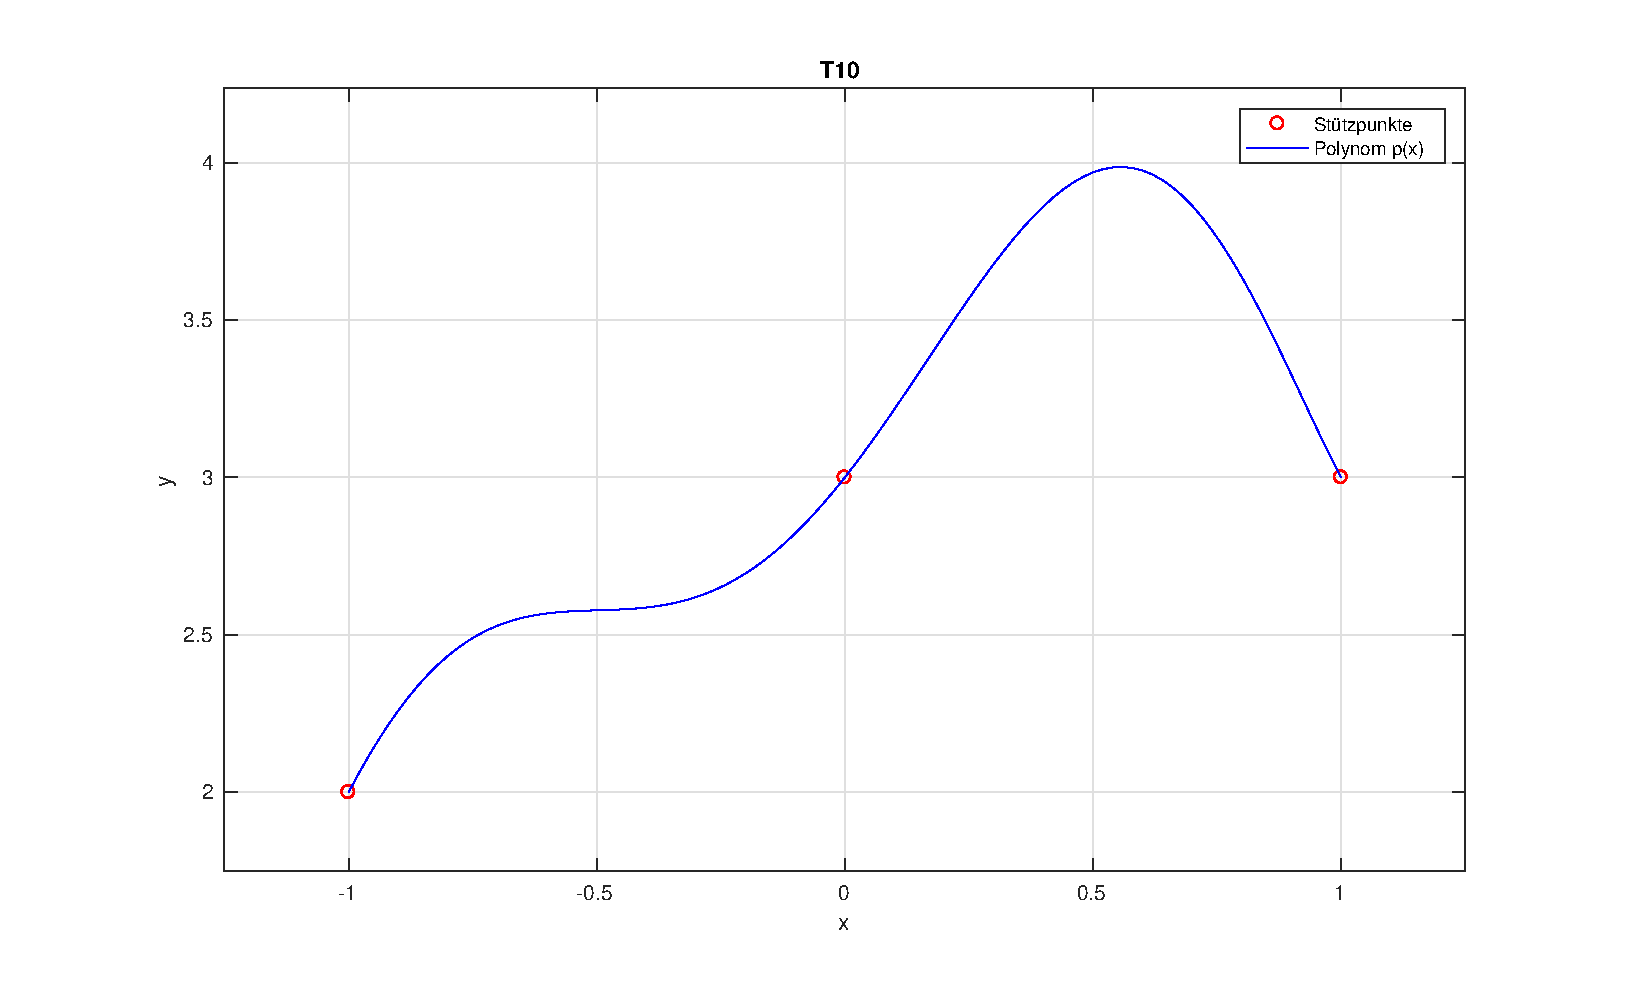
\includegraphics[width=1.0\textwidth]{T10}
		\caption{T10 \, Stützpunkte und Interpolationspolynom $p(x)$}
	\end{figure}
	\newpage
	
	\paragraph{T11}\mbox{}\\
	\textbf{%
		a) Schreiben Sie für natürliche Splines das zugehörige lineare Gleichungssystem für die Momente $\pmb{M_0, \dots, M_n}$ in Matrizen-Schreibweise an.
	}\\
		Nach Definition 3.9, S. 62:\\
		$\mbox{}\quad$ Natürlicher Spline: $s''(x_0)=s(x_n)=0$ \\
		$\mbox{}\quad$ Die Momente an beiden Enden des Balken sind 0 $\Rightarrow (3.90) M_0=0 \text{ und } M_n=0$ \\
		Das hergeleitete lineare Gleichungssystem für die Momente $M_i$ lautet
		\begin{align*}
			\frac{h_i}{6}M_i+\frac{h_i+h_{i+1}}{3}M_{i+1}+\frac{h_{i+1}}{6}M_{i+2} 
				= \frac{y_{i+2}-y_{i+1}}{h_{i+1}}-\frac{y_{i+1}-y_i}{h_i}, \quad i = 0,\dots n-2
		\end{align*}
		Bsp. n=7 \\
		Um die Form einer Tridiagonalmatrix zu erreichen, müssen $M_0$ und $M_7$ gestrichen werden.
		\begin{align*}\frac{1}{6}
		\begin{bmatrix}
			\cancel{h_0 M_0}+2(h_0+h_{1})M_{1}+h_{1} M_{2} \\
			h_1 M_1+2(h_1+h_{2})M_{2}+h_{2} M_{3} \\
			h_2 M_2+2(h_2+h_{3})M_{3}+h_{3} M_{4} \\
			h_3 M_3+2(h_3+h_{4})M_{4}+h_{4} M_{5} \\
			h_4 M_4+2(h_4+h_{5})M_{5}+h_{5} M_{6} \\
			h_5 M_5+2(h_5+h_{6})M_{6}+\cancel{h_{6} M_{7}}
		\end{bmatrix} = \frac{1}{6} 
		\begingroup % keep the change local
		\setlength\arraycolsep{0pt}
		\begin{bmatrix}
			2(h_0+h_1) & h_1        & 0          & 0          & 0          & 0          \\
			h_1        & 2(h_1+h_2) & h_2        & 0          & 0          & 0          \\
			0          & h_2        & 2(h_2+h_3) & h_3        & 0          & 0          \\
			0          & 0          & h_3        & 2(h_3+h_4) & h_4        & 0          \\
			0          & 0          & 0          & h_4        & 2(h_4+h_5) & h_5        \\
			0          & 0          & 0          & 0          & h_5        & 2(h_5+h_6)
		\end{bmatrix}
		\endgroup
			\begin{bmatrix}
				\cancel{M_0} \\
				M_1 \\
				M_2 \\
				M_3 \\
				M_4 \\
				M_5 \\
				M_6 \\
				\cancel{M_7}
			\end{bmatrix}
			=
			\begin{bmatrix}
				\frac{y_2-y_1}{h_1}-\frac{y_1-y_0}{h_0} \\
				\frac{y_3-y_2}{h_2}-\frac{y_2-y_1}{h_1} \\
				\frac{y_4-y_3}{h_3}-\frac{y_3-y_2}{h_2} \\
				\frac{y_5-y_4}{h_4}-\frac{y_4-y_3}{h_3} \\
				\frac{y_6-y_5}{h_5}-\frac{y_5-y_4}{h_4} \\
				\frac{y_7-y_6}{h_6}-\frac{y_6-y_5}{h_5}
			\end{bmatrix}
		\end{align*}
		Allgemein
		\begin{align*}
		\frac{1}{6} 
		\begingroup % keep the change local
		\setlength\arraycolsep{3pt}
		\setstretch{2.0}
		\begin{bmatrix}
			2(h_0+h_1) & h_1        & 0          &        &                &         &         &                    &  \\
			h_1        & 2(h_1+h_2) & h_2        & 0      &                &         &         &                    &  \\
			0          & h_2        & 2(h_2+h_3) & h_3    & 0              &         &         &                    &  \\
			           & \ddots     & \ddots     & \ddots & \ddots         & \ddots  &         &                    &  \\
			           &            & 0          & h_i    & 2(h_i+h_{i+1}) & h_{i+1} & 0       &                    &  \\
			           &            &            & \ddots & \ddots         & \ddots  & \ddots  & \ddots             &  \\
			           &            &            &        &                & 0       & h_{n-3} & 2(h_{n-3}+h_{n-2}) & h_{n-2}            \\
			           &            &            &        &                &         & 0       & h_{n-2}            & 2(h_{n-2}+h_{n-1})
		\end{bmatrix}
		\endgroup
		\begin{bmatrix}
			M_1     \\
			M_2     \\
			M_3     \\
			\vdots  \\
			M_i     \\
			\vdots  \\
			M_{n-2} \\
			M_{n-1}
		\end{bmatrix}
		=
		\begin{bmatrix}
			\frac{y_{2}-y_{1}}{h_{1}}-\frac{y_{1}-y_{0}}{h_0}               \\
			\frac{y_{3}-y_{2}}{h_{2}}-\frac{y_{2}-y_{1}}{h_1}               \\
			\frac{y_{4}-y_{3}}{h_{3}}-\frac{y_{3}-y_{2}}{h_2}               \\
			\vdots                                                          \\
			\frac{y_{i+2}-y_{i+1}}{h_{i+1}}-\frac{y_{i+1}-y_i}{h_i}         \\
			\vdots                                                          \\
			\frac{y_{n-1}-y_{n-2}}{h_{n-2}}-\frac{y_{n-2}-y_{n-3}}{h_{n-3}} \\
			\frac{y_{n}-y_{n-1}}{h_{n-1}}-\frac{y_{n-1}-y_{n-2}}{h_{n-2}}
		\end{bmatrix}
		\end{align*}	
	\newpage
	\textbf{%
		b) Stellen Sie die beiden "fehlenden" Gleichungen für die Momente $\pmb{M_0, \dots, M_n}$ für periodische Splines mit $\pmb{s(x_0) = s(x_n)}$, $\pmb{s′(x_0) = s′(x_n)}$ und $\pmb{s''(x_0)=s''(x_n)}$ auf. \\
		Wie sieht die Matrix des gesamten Gleichungssystems aus? Ist sie auch eine Tridiagonalmatrix?
	}
		Auf S. 65 wird darauf hingewiesen, dass $s(x_0)=s(x_n)$ keine Bedingung für das Gleichungssystem ist. Die Punkte müssen bereits so gegeben sein! D.h. $s(x_0)=\underline{y_0=y_n}=s(x_n)$.
		\begin{align}\tag{3.38}
			s''_i(x)&=M_i+\frac{M_{i+1}-M_i}{h_i}(x-x_i), \quad x \in [x_i, x_{i+1}], \quad i=0,\dots,n-1
        \end{align}
        Einsetzen von $s''(x_0)=s''(x_n)$ in 3.38
        \begin{align*}
			s''_0(x_0)&=M_0+\frac{M_{1}-M_0}{h_0}(x_0-x_0) = M_1 \\ s''_{n-1}(x_n)&=M_{n-1}+\frac{M_{n}-M_{n-1}}{h_{n-1}}(x_n-x_{n-1}) \\
            \\
            M_1 &= M_{n-1}+\frac{M_{n}-M_{n-1}}{h_{n-1}}(x_n-x_{n-1}) \\
            0 &= M_{n-1}+\frac{M_{n}-M_{n-1}}{h_{n-1}}(x_n-x_{n-1})-M_1
		\end{align*}
        Für $s′(x_0) = s′(x_n)$ muss in die Integrierte Gleichung
        \begin{align}\tag{3.82}
            s'_i(x)=M_i(x-x_i)+\frac{M_{i+1}-M_i}{2h_i}(x-x_i)^2+C_i
        \end{align}
        die Konstante $C_i$ eingesetzt werden
        \begin{align}\tag{3.84}
            C_i=\frac{y_{i+1}-y_i}{h_i}-\frac{h_i}{6}(2M_i+M_{i+1}).
        \end{align}
        Einsetzen in $s′(x_0) \text{ und } s′(x_n)$
        \begin{align*}
            s'_i(x)&=M_i(x-x_i)+\frac{M_{i+1}-M_i}{2h_i}(x-x_i)^2+\frac{y_{i+1}-y_i}{h_i}-\frac{h_i}{6}(2M_i+M_{i+1}) \\
            s'_0(x_0)&=M_0(x_0-x_0)+\frac{M_1-M_0}{2h_0}(x_0-x_0)^2+\frac{y_1-y_0}{h_0}-\frac{h_0}{6}(2M_0+M_1) \\
            s'_0(x_0)&=\frac{y_1-y_0}{h_0}-\frac{h_0}{6}(2M_0+M_1) \\
            s_{n-1}′(x_n)&=M_{n-1}(x_n-x_{n-1})+\frac{M_n-M_{n-1}}{2h_{n-1}}(x_n-x_{n-1})^2+\frac{y_n-y_{n-1}}{h_{n-1}}-\frac{h_{n-1}}{6}(2M_{n-1}+M_n) \\
            s_{n-1}′(x_n)&=M_{n-1}h_{n-1}+\frac{M_n-M_{n-1}}{2h_{n-1}}h_{n-1}^2+\frac{y_n-y_{n-1}}{h_{n-1}}-\frac{h_{n-1}}{6}(2M_{n-1}+M_n) \\
            s_{n-1}′(x_n)&=\frac{h_{n-1}}{2}(M_{n-1}+M_n)+\frac{y_n-y_{n-1}}{h_{n-1}}-\frac{h_{n-1}}{6}(2M_{n-1}+M_n) \\
            s_{n-1}′(x_n)&=\frac{h_{n-1}}{6}\left(3M_{n-1}+3M_n-2M_{n-1}+M_n\right)+\frac{y_n-y_{n-1}}{h_{n-1}}  \\
            s_{n-1}′(x_n)&=\frac{h_{n-1}}{6}\left(M_{n-1}+4M_n\right)+\frac{y_n-y_{n-1}}{h_{n-1}} 
        \end{align*}
        Gleichsetzen
        \begin{align*}
            \frac{y_1-y_0}{h_0}-\frac{h_0}{6}(2M_0+M_1) &= \frac{h_{n-1}}{6}\left(M_{n-1}+4M_n\right)+\frac{y_n-y_{n-1}}{h_{n-1}}  \\
           -\frac{h_0}{6}(2M_0+M_1)-\frac{h_{n-1}}{6}\left(M_{n-1}+4M_n\right)
            &=
            \frac{y_n-y_{n-1}}{h_{n-1}}-\frac{y_1-y_0}{h_0}
        \end{align*}
        Nun verwenden wir $s(x_n)=s(x_0) \rightarrow y_{n}=y_0$ und $s''(x_n)=s''(x_0) \rightarrow M_n=M_0$.
        \begin{align*}
            -\frac{h_0}{6}(2M_0+M_1)-\frac{h_{n-1}}{6}\left(M_{n-1}+4M_0\right)
            &=
            \frac{y_0-y_{n-1}}{h_{n-1}}-\frac{y_1-y_0}{h_0}
        \end{align*}
\end{document}